\documentclass[a4paper, 12pt,]{scrartcl}



\usepackage[utf8]{inputenc}

\usepackage[ngerman]{babel}
\usepackage{amssymb}
\usepackage[T1]{fontenc}
\usepackage{mathtools}
\usepackage{amsmath}
\usepackage{ntheorem}
\usepackage{bbm}
\usepackage{dsfont}
\usepackage{color}
\usepackage{slashed}
\usepackage{hyperref}
\usepackage{graphicx} 
\usepackage{bm}
\usepackage{mathabx}
\usepackage{float}
\usepackage{mwe}
\usepackage{multirow}
\begin{document}
\begin{titlepage}
	\centering
	{\scshape\LARGE Universität Tübingen \par}
	\vspace{2cm}
	{\huge\bfseries Elektrische Resonanz \par}
	\vspace{2cm}
	{\Large \scshape Blockpraktikum 2021} \par
	\vspace{2cm}
	{\Large  Erste Version} \par
	\vspace{2cm}
	{\Large\itshape \underline{Christian Gommeringer} \space \space  \underline{Matthias Gatter}\par}
	\vfill 
	{\large unter der Betreuung von Dr. Hehl}
	\vfill

	{\large \today\par}
\end{titlepage}
\newpage 
\tableofcontents 

\newpage
\section{Einleitung}
\begin{flushleft}
Dieser Versuch thematisiert das Resonanzverhalten drei verschiedener Schaltungen: des Schwingkreises, des Parallelkreises 1. Ordnung und des Parallelkreises 2. Ordnung. Die Strom und Spannungsmessung nehmen wir in diesem Experiment durch ein analoges Oszilloskop und das Cassy Messsystem durch.

\end{flushleft}
% > < | 
\section{Theorie}
Zunächst behandeln wir den theoretischen Zusammenhang zwischen Spannung und Strom in diesen Schaltungen. Als erstes befassen wir uns mit dem Schwingkreis
\begin{figure}[H]\centering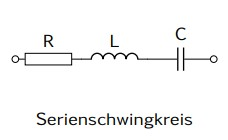
\includegraphics[scale=1]{SeSK}\caption{Schaltungsaufbau eines Schwingkreises}\end{figure}
In einer Schaltung wie dieser teilt sich der Spannungsabfall auf die einzelnen Komponenten auf. Es gelten die folgenden Relationen für die einzelnen Komponenten.
\begin{align*}U_{R}=&I\cdot{R}\\
U_L=&L\cdot\dot{I}\:\text{mit der Induktivität }L\\
Q=&C\cdot{U_C}\:\text{mit der Kapazität }C\\
\Rightarrow\;I=&C\,\dot{U}_C\end{align*}
Zu beachten ist, dass $U_L$ und $U_C$ der externen Spannungsquelle entgegen wirken. 
\begin{gather*}U_{ex}-U_L-U_C=U_R\\
\Rightarrow\;\dot{U}_{ex}=\dot{U}_R+\dot{U}_L+\dot{U}_C\end{gather*}
Für ein Spannungssignal der Form $U_{ex}=U_0\,\sin(\omega{t})$ ergibt sich folgende Differentialgleichung.
\begin{equation*}\omega\,{U_0}\,\cos\omega{t}=R\,\dot{I}+L\,\ddot{I}+\frac{1}{C}\,I\end{equation*}
Diese Gleichung hat folgende Lösung
\begin{equation*}I(t)=e^{-\frac{R}{2L}\,t}\,\left(B\,e^{i\,\sqrt{\frac{1}{L\,C}-\frac{R^2}{4\,L^2}}\,t}+D\,e^{-i\,\sqrt{\frac{1}{L\,C}-\frac{R^2}{4\,L^2}}\,t}\right)+A\,\cos(\omega{t}+\varphi),\end{equation*}
wobei B und D Konstanten sind, die durch die Anfangsbedingungen bestimmt sind. Für diese Teil der Lösung interessieren wir uns allerdings nicht, da wir unsere Messung erst nach einer gewissen Einschwingzeit vornehmen, nach der der erste Term effektiv verschwunden ist. Deshalb bestimme ich diese Konstanten hier auch nicht näher. Die signifikanten Konstanten A und $\varphi$ müssen folgende Gleichung erfüllen.
\begin{align*}\omega\,U_0=A\,e^{i,\varphi}\,\left(i\,R\,\omega-L\,\omega^2+\frac{1}{C}\right)\\
\Rightarrow\;A=&\frac{\omega\,U_0}{\sqrt{R^2\,\omega^2+\left(\frac{1}{C}-L\,\omega^2\right)^2}}\\
\tan\varphi=&-\frac{R\,\omega}{\frac{1}{C}-L\,\omega^2}\end{align*}
Nach ausreichend langer Zeit $t>>2L/R$ stellt sich dann die Beziehung zwischen Spannung und Strom ein von
\begin{align*}I(t)=&\mathfrak{Im}\left[i\,\frac{\omega\,U_0}{\sqrt{R^2\,\omega^2+\left(\frac{1}{C}-L\,\omega^2\right)^2}}\,e^{i\,(\omega{t}+\varphi)}\right]\\
=&\mathfrak{Im}\left[Z\,U_0\,e^{i\,\omega\,t}\right]\:\text{mit}\\
|Z|=&\frac{U_0}{A}=\sqrt{R^2+\left(\frac{1}{C\,\omega}-L\,\omega\right)^2}\quad\text{und}\\
\text{arg}(Z)=&-\varphi+\frac{\pi}{2}\end{align*}

Als nächstes untersuchen wir den Parallelkreis erster Ordnung
\begin{figure}[H]\centering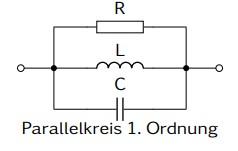
\includegraphics[scale=1]{PK 1}\caption{Schaltungsaufbau eines Parallelkreises 1. Ordnung}\end{figure}
Nach der Maschenregel liegt an jedem Zweig die selbe Spannung an
\begin{align*}U_{ex}&=I_R\,R\\
U_{ex}&=I_L\,R_L+U_L=I_L\,R+L\,\dot{I}\\
U_{ex}&=I_C\,R_C+U_C\,\Rightarrow\;\dot{U}_{ex}=\dot{I}_C\,R_C+\frac{1}{C}\,I_C\end{align*}
Zur Vereinfachung setzen wir $R_L$ und $R_C$ auf 0. Damit lassen sich die Ströme leicht angeben
\begin{align*}I_R&=\frac{U_0}{R}\,\sin\omega{t}\\
I_L&=-\frac{U_0}{L\,\omega}\,\cos\omega{t}\\
I_C&=U_0\,\omega\,C\,\cos\omega{t}\end{align*}
Daraus lässt sich wiederum die Impedanz ableiten
\begin{align*}I_\text{ges}&=\frac{U_0}{R}\,\sin\omega{t}-\frac{U_0}{L\,\omega}\,\cos\omega{t}+U_0\,\omega\,C\,\cos\omega{t}\\
&=\mathfrak{Im}\left[\left(\frac{1}{R}-i\,\frac{1}{L\,\omega}+i\,\omega\,C\right)\,U_0\,e^{i\,\omega\,t}\right]\\
&=\mathfrak{Im}\left[\frac{1}{Z}\,U_0\,e^{i\,\omega\,t}\right]\quad\text{mit}\\
|Z|&=\frac{R\,L\,\omega}{\sqrt{L^2\,\omega^2+R^2\,(L\,\omega^2\,C-1)^2}}\quad\text{und}\\
\tan(\text{arg}(Z))&=R(\omega\,C-\frac{1}{L\,\omega})\end{align*}

Für den Parallelkreis 2. Ordnung können wir ähnlich vorgehen.
\begin{figure}[H]\centering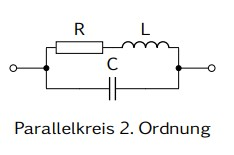
\includegraphics[scale=1]{PK 2}\caption{Schaltungsaufbau eines Parallelkreises 2. Ordnung}\end{figure}
Über die Zusammenhänge mit der angelegten Spannung
\begin{align*}U_{ex}&=U_R+U_L=(R+R_L)\,I_L+L\,\dot{I}_L\\
\dot{U}_{ex}&=\dot{I}_C\,R_C+\frac{1}{C}\,I_C,\end{align*}
wobei wir $R_L$ und $R_C$ wieder auf Null setzen, können wir den Strom für die einzelnen Zweige berechnen. Für den Strom am Kondensator gilt wie oben
\begin{equation*}I_C=U_0\,\omega\,C\,\cos\omega{t}\end{equation*}
Für den Strom an Widerstand und Spule ergibt sich
\begin{equation*}I_L(t)=B\,e^{-\frac{R}{L}\,t}+A'\,\sin(\omega\,t+\varphi')\end{equation*}
B kann wieder durch die Anfangsbedingungen bestimmt werden. Für A' und $\varphi'$ gilt folgende Gleichung.
\begin{align*}U_0=A'\,e^{i\,\varphi'}\,(R+i\,\omega\,L)\\
\Rightarrow\;A'&=\frac{U_0}{\sqrt{R^2+\omega^2\,L^2}}\\
\tan\varphi'&=-\frac{\omega\,L}{R}\end{align*}
Daraus berechnet sich die Impedanz auf folgende Weise
\begin{align*}I_\text{ges}(t)&=U_0\,\omega\,C\,\cos\omega{t}+\frac{U_0}{\sqrt{R^2+\omega^2\,L^2}}\,\sin(\omega\,t+\varphi')\\
&=\mathfrak{Im}\left[\left(i\,\omega\,C+\frac{1}{\sqrt{R^2+\omega^2\,L^2}}\,e^{i\,\varphi'}\right)\,U_0\,e^{i\,\omega\,t}\right]\\
&=\mathfrak{Im}\left[\frac{1}{Z}\,U_0\,e^{i\,\omega\,t}\right]\end{align*}
Für die Impedanz Z gilt damit
\begin{align*}
|Z|&=\sqrt{\frac{R^2+\omega^2\,L^2}{R^2\,\omega^2\,C^2+(\omega^2\,L\,C-1)^2}}\\
\tan(\text{arg}(Z))&=-\frac{\omega}{R}\,(C\,(R^2+\omega^2\,L^2)-L)\end{align*}
Wie auch gleich gezeigt wird, haben die Amplituden der abgeleiteten Impedanzen alle eine resonanzfähige Form. Zunächst bestimme ich die Resonanzfrequenz des Schwingkreises $\omega_{S,0}$.
\begin{align*}0\overset{!}{=}\frac{\partial{|Z_S|}}{\partial\omega}=\frac{-\frac{1}{C^2\,\omega^3}+L^2\,\omega}{\sqrt{R^2+\left(\frac{1}{C\,\omega}-L\,\omega\right)^2}}\\
\Rightarrow\,\frac{1}{\omega^3}\,(L^2\,\omega^4-\frac{1}{C^2})\overset{!}{=}0\\
\Rightarrow\,\omega_{S,0}=\frac{1}{\sqrt{L\,C}}\end{align*}
Für die Impedanz des Parallelkreises 1. Ordnung 
\begin{equation*}|Z_{P1}|=\frac{R\,L\,\omega}{\sqrt{L^2\,\omega^2+R^2\,(L\,\omega^2\,C-1)^2}}\end{equation*}
berechnet sich $\omega_{P1,0}$ durch
\begin{align*}0\overset{!}{=}\frac{\partial{|Z_{P2}|^2}}{\partial\omega}=R\,L\,\frac{R^2-R^2\,L^2\,C^2\,\omega^4}{\sqrt{L^2\,\omega^2+R^2\,(L\,\omega^2\,C-1)^2}}\\
\Rightarrow\;\omega_{P1,0}=\frac{1}{\sqrt{L\,C}}\end{align*}
Für die den Parallelkreis 2. Ordnung gestaltet sich die Bestimmung der Resonanzfrequenz etwas schwieriger, da hier die Nullstellen eines Polynoms 4. Grades ermittelt werden müssen. Die numerische bestimmte Lösung ist
\begin{align*}\omega_{P2,0}=&\sqrt{\frac{\sqrt{L^6+2\,C\,L^5\,R^2}-C\,L^2\,R^2}{C\,L^4}}\\
=&\sqrt{\frac{\sqrt{L^2+2\,C\,L\,R^2}-C\,R^2}{C\,L^2}}\end{align*}
Hierbei erkennt man, dass bei der Resonanzfrequenz in diesem Fall noch eine Phasenverschiebung auftritt, während bei den ersten beiden Fällen die Phasenverschiebung in der Resonanz immer 0 war. Im Parallelkreis 2. Ordnung ist die Frequenz für die es keine Phasenverschiebung gibt
\begin{equation*}\omega_{\text{arg}(Z)=0}=\sqrt{\frac{1}{L\,C}-\frac{R^2}{L^2}}\neq\omega_{P2,0}\end{equation*}

\section{Durchführung}
Im ersten Teil der Messung vermaßen wir den Schwingkreis erster Ordnung mit Hilfe eines Oszilloskops. Die Daten des Schwingkreises waren $C=4.99\,nF$, $L=314.8\,mH$ und $R=14.76\,\Omega$. Zur Messung schalteten wir den Schwingkreis in Reihe mit einem verstellbaren Widerstand, den wir auf $R_\text{pot}=22\,k\Omega$ einstellten, und griffen die Spannung am Potentiometers sowie am Schwingkreis ab, welche wir als Spannung an die y- und x-Ablenkplatten des Oszilloskops legten. Die Trajektorie, die vom Elektronenstrahl abgebildet wurde, beschrieb damit eine Ellipse, deren Form von der Phasenverschiebung zwischen $U_x$ und $U_y$ abhing. Da gilt $U_y=I\,R_\text{pot}$, entspricht diese Phasenverschiebung auch jener zwischen Strom und Spannung am Schwingkreis. Die Skalen der x- und y-Achse stellten wir so ein, dass sowohl $U_{x,\text{max}}$ als auch $U_{y,\text{max}}$ die gleiche Längeneinheit $Z_0$ einnahm. Über die Verzerrungsfaktoren $p_x$ und $p_y$ lassen sich über $U_{x,\text{max}}=p_x\,Z_0$ und $U_{y,\text{max}}=p_y\,Z_0$ wieder die ursprünglichen Werte erhalten. Der Betrag der Impedanz lässt sich daraus direkt bestimmen
\begin{equation*}|Z|=\frac{U_\text{max}}{I_\text{max}}=\frac{U_{x,\text{max}}}{U_{y,\text{max}}/R_\text{pot}}=\frac{p_x}{R_\text{pot}\,p_y}\end{equation*}
Für die Phasenverschiebung sind die Überlegungen etwas aufwändiger. Eine Ellipse lässt sich im Allgemeinen durch
\begin{equation*}\vec{r}=\left(\begin{array}{c}a\,\cos(\varphi)\\ b\,\sin(\varphi)\end{array}\right)\end{equation*}
beschreiben, wobei a die große und b die kleine Halbachse darstellen. Die Form der Ellipse ändert sich natürlich nicht, wenn wir den Winkel um eine bestimmte Phase verschieben.
\begin{equation*}\vec{r}=\left(\begin{array}{c}a\,\cos(\varphi-\alpha_m)\\ b\,\sin(\varphi-\alpha_m)\end{array}\right)\end{equation*}
beschriebt immer noch eine Ellipse der gleichen Form (a,b). Wenn wir diese Verschiebung des Startpunkts als eine Drehung des Koordinatensystems verstehen, das dann mit dem Koordinatensystem auf Oszilloskop übereinstimmen soll, muss gelten
\begin{align*}\vec{r}^2(\varphi=0)=Z_0^2=\vec{r}^2(\varphi=\frac{\pi}{2})\\
a^2\,\cos^2(\alpha_m)+b^2\,\sin^2(\alpha_m)=a^2\,\sin^2(\alpha_m)+b^2\,\cos^2(\alpha_m)\\
a^2\,(\cos^2(\alpha_m)-\sin^2(\alpha_m))=b^2(\cos^2(\alpha_m)-\sin^2(\alpha_m)),\end{align*}
was nur gelten kann ($a\neq{b}$), wenn
\begin{align*}\cos(\alpha_m)=&\sin(\alpha_m)\\
\Rightarrow\;\alpha_m=&\frac{\pi}{4}\cdot{n}\,\pi\;n\in\mathbb{N}\end{align*}
Damit gilt, dass in den Scheitelpunkten der Ellipse $U_x=U_y$. Für Spannungstrajektorien der Form 
\begin{align*}U_x=Z_0\,\sin(\varphi)\\
U_y=Z_0\,\sin(\varphi+\theta)\end{align*}
gibt es für diese Bedingungen z.B. die Punkte
\begin{align*}
\varphi_a&=\frac{\pi}{2}-\frac{\theta}{2}\quad\rightarrow\;a\\
\varphi_b&=-\frac{\theta}{2}\quad\rightarrow\;b\end{align*}
Es gilt
\begin{align*}
a^2&=2\,Z_0^2\,\sin^2(\frac{\pi}{2}-\frac{\theta}{2})\\
a&=\sqrt{2}\,Z_0\,\cos(\frac{\theta}{2})\\
b&=\sqrt{2}\,Z_0\,\sin(\frac{\theta}{2})\\
\Rightarrow\;\frac{b}{a}&=\tan(\frac{\theta}{2})
\end{align*}
Wir führten die oben beschriebene Messung für verschieden Frequenzen der Wechselspannung durch
\begin{table}[H]\centering\begin{tabular}{ |c | c | c | c | c | c | c | c | c | }\hline
Frequenz in Hz&500.3&	1001&	1500&	2000.2&	2501.7&	3000.6&	3500.1&	4000.2\\\hline\hline
a&3.1	&3.14	&3.26	&3.35	&3.5	&3.7	&4	&4.2\\\hline
b&2.9	&2.83	&2.77	&2.65	&2.4	&2.05	&1.85	&0.05\\\hline
$p_x$&0.2	&0.5	&0.5	&0.5	&1	&1	&1	&1\\\hline
$p_y$&1	&1	&1	&1	&0.5	&0.5	&0.5	&2\\\hline
\multicolumn{9}{c}{}\\\hline
Frequenz in Hz&	4500.5&	5000.1	&5500.1&	6000&	6499.4	&6999.9	&7500.3	&8000.1\\\hline\hline
a&4.05	&3.8	&3.7	&3.6	&3.45	&3.5	&3.45	&3.4\\\hline
b&1.2	&1.75	&2.45	&2.25	&2.35	&2.35	&2.4	&2.45\\\hline
$p_x$&1	&1	&1	&0.5	&0.5	&0.5	&0.5	&0.5\\\hline
$p_y$&0.2	&0.5	&0.5	&0.2	&0.2	&0.5	&0.5	&0.5\\\hline\end{tabular}
\caption{Vermessung des Parallelkreises 1. Ordnung mit Oszilloskop}\end{table}




\end{document}